\subsection[Umsetzung eines kanalbasieren Systemes]{Umsetzung eines kanalbasieren Systemes am Beispiel von Scribe}
\label{chap:related:scribe}
Eine Umsetzung von Publish/Subscribe-Systemen in verteilen Systemen, ist der Aufbau eines Multicast-Trees\index{Multicast-Tree}, d.h. eines durch die Knoten im Netz gebildeten Baumes in dem die Nachrichten verteilt werden. Hierbei wird pro Kanal ein eigener Multicast-Tree aufgebaut. Am Algorithmus von Scribe \cite{Castro2002Scribe}wird diese Struktur beschrieben.

Scribe basiert auf dem strukturierten Overlay-Netzwerk Pastry \cite{Rowstron2001} und erzeugt einen vom Subscriber zum Publischer aufgebauten Baum \emph{reverse path forwarding tree} \cite{Dalal1978}.

\begin{figure}[htbp]
\centering
\resizebox{\textwidth}{!}{%
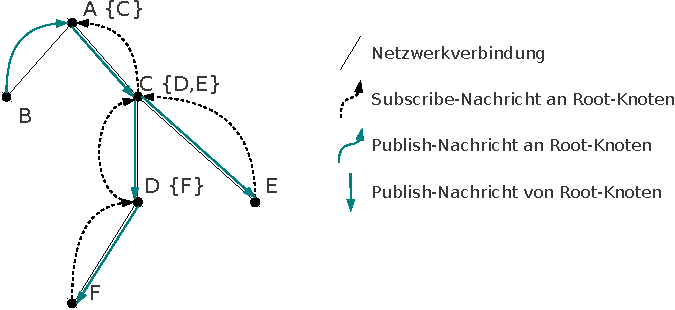
\includegraphics{grafics/multicast_tree.pdf}}
\caption{Schema eines Multicast-Trees}
\label{fig:multicast_tree}
\end{figure}

\Fref{fig:multicast_tree} zeigt ein Netzwerk mit den sechs Knoten A-F. Die Verbindungen der Knoten werden durch dünne schwarze Linien dargestellt. Beispielsweise hat Knoten C Verbindungen zu A, B, D und F.\\
Der Multicast-Tree benötigt einen Knoten, der die Wurzel (im Folgenden \emph{Root-Knoten} genannt) darstellt. Aus Hashwert des Kanalnamens wird ein Schlüssel berechnet. Derjenige Knoten, der aufgrund der Netzwerkmetrik für diesen Schlüssel zuständig ist, wird Root-Knoten des Kanals. Im abgebildeten Falle ist dies Knoten A.\\
Weiterhin hält jeder Knoten eine Liste bei ihm angemeldeter Knoten. In der Abbildung wird diese Liste durch geschweifte Klammern nach der Knotenbezeichnung dargestellt.

\paragraph{Subscribe}
Knoten F sendet eine \emph{subscribe}-Nachricht an A. Diese Nachrichten sind in der Grafik durch gebogene gestrichelte schwarze Verbindungslinien mit Pfeil dargestellt. Das Netzwerk würde diese Nachricht über Knoten D und C an A routen. Knoten D lässt die Nachricht terminieren und trägt F in die Liste der Subscriber ein. Knoten D sendet nun selbst eine subscribe-Nachricht an A. C, über den die Nachricht geroutet wird, terminiert diese, trägt D in die Liste ein und sendet selbst eine subscribe-Nachricht an A. A erhält nun diese Nachricht und trägt C in die Liste ein. Damit sind nun insgesamt drei Nachrichten verschickt worden.\\
Wenn sich Knoten E für den Kanal einschreibt, wird die subscribe-Nachricht an A über den Knoten C geleitet. Dieser terminiert die Nachricht und fügt E der Liste hinzu. Da C selbst angemeldet ist, muss keine weitere Nachricht versendet werden.

Scribe fordert periodische Anmeldungen zur Erhöhung der Fehlertoleranz. Ist ein Knoten ausgefallen, routet das Netzwerk die Nachrichten über andere Knoten. Damit kann der Multicast-Tree wieder aufgebaut werden.

\paragraph{Unsubscribe}
Der Austritt aus einem Kanal erfolgt ähnlich zur Anmeldung. Die Nachricht läuft nur bis zum nächsten Knoten und terminiert dort. Der Knoten entfernt den Sender der Nachricht aus seiner Liste und sendet selbst nur eine \emph{unsubscribe}-Nachricht, wenn die Liste leer ist und er selbst nicht angemeldet ist.

\paragraph{Publish}
In \Fref{fig:multicast_tree} möchte Knoten B eine Nachricht im Kanal publizieren. B sendet darauf eine Nachricht an den Root-Knoten A, da dieser für diesen Kanal zuständig ist (gebogene türkise Linie). Nun sendet A diese Nachricht an alle Knoten in seiner Liste (gerader türkise Linie mit Pfeil). Dies ist in der Abbildung nur Knoten C. Dieser sendet sie weiter an D und E. E gibt diese Nachricht direkt an die Applikation weiter, während D die Nachricht an F schicken muss.


Hierbei ist klar ersichtlich, dass zusätzliche Nachrichten verteilt werden müssen, wenn Knoten F eine Nachricht im Kanal publizieren möchte. Diese Nachricht muss erst von Knoten F zu Knoten A wandern, damit A diese Nachricht wieder über die anderen Knoten zurücksendet. Optimierte Versionen dieses Algorithmus können hier ansetzen und zu publizierende Nachrichten nicht mehr an den Knoten senden, der ihnen diese Nachricht geschickt hat. So würde C die Nachricht nur noch an E weiterleiten.

Bayeux \cite{Zhuang2001} ist ein ähnliches System, jedoch auf Basis des Overlay-Netzwerkes Tapestry \cite{Zhao2004Tapestry}. Tapestry entspricht auch der generischen API, somit stellt dies keinen Unterschied zu Pastry dar. Im Gegensatz zu Scribe, wird bei Bayeux der Multicast-Tree vom Root-Knoten aus aufgebaut. Aufgrund der unterliegenden Routingstruktur des genutzten Overlay-Netzwerkes können sich diese Pfade unterscheiden.
